\documentclass{standalone}\usepackage[]{graphicx}\usepackage[]{color}
%% maxwidth is the original width if it is less than linewidth
%% otherwise use linewidth (to make sure the graphics do not exceed the margin)
\makeatletter
\def\maxwidth{ %
  \ifdim\Gin@nat@width>\linewidth
    \linewidth
  \else
    \Gin@nat@width
  \fi
}
\makeatother

\definecolor{fgcolor}{rgb}{0.345, 0.345, 0.345}
\newcommand{\hlnum}[1]{\textcolor[rgb]{0.686,0.059,0.569}{#1}}%
\newcommand{\hlstr}[1]{\textcolor[rgb]{0.192,0.494,0.8}{#1}}%
\newcommand{\hlcom}[1]{\textcolor[rgb]{0.678,0.584,0.686}{\textit{#1}}}%
\newcommand{\hlopt}[1]{\textcolor[rgb]{0,0,0}{#1}}%
\newcommand{\hlstd}[1]{\textcolor[rgb]{0.345,0.345,0.345}{#1}}%
\newcommand{\hlkwa}[1]{\textcolor[rgb]{0.161,0.373,0.58}{\textbf{#1}}}%
\newcommand{\hlkwb}[1]{\textcolor[rgb]{0.69,0.353,0.396}{#1}}%
\newcommand{\hlkwc}[1]{\textcolor[rgb]{0.333,0.667,0.333}{#1}}%
\newcommand{\hlkwd}[1]{\textcolor[rgb]{0.737,0.353,0.396}{\textbf{#1}}}%

\usepackage{framed}
\makeatletter
\newenvironment{kframe}{%
 \def\at@end@of@kframe{}%
 \ifinner\ifhmode%
  \def\at@end@of@kframe{\end{minipage}}%
  \begin{minipage}{\columnwidth}%
 \fi\fi%
 \def\FrameCommand##1{\hskip\@totalleftmargin \hskip-\fboxsep
 \colorbox{shadecolor}{##1}\hskip-\fboxsep
     % There is no \\@totalrightmargin, so:
     \hskip-\linewidth \hskip-\@totalleftmargin \hskip\columnwidth}%
 \MakeFramed {\advance\hsize-\width
   \@totalleftmargin\z@ \linewidth\hsize
   \@setminipage}}%
 {\par\unskip\endMakeFramed%
 \at@end@of@kframe}
\makeatother

\definecolor{shadecolor}{rgb}{.97, .97, .97}
\definecolor{messagecolor}{rgb}{0, 0, 0}
\definecolor{warningcolor}{rgb}{1, 0, 1}
\definecolor{errorcolor}{rgb}{1, 0, 0}
\newenvironment{knitrout}{}{} % an empty environment to be redefined in TeX

\usepackage{alltt}
\usepackage{tikz}
 
 
\newcommand\commit[2]{\node[commit] (#1) {}; \node[clabel] at (#1) {\texttt{#1}: #2};}
\newcommand\ghost[1]{\coordinate (#1);}
\newcommand\connect[2]{\path (#1) to[out=90,in=-90] (#2);}
\IfFileExists{upquote.sty}{\usepackage{upquote}}{}
\begin{document}

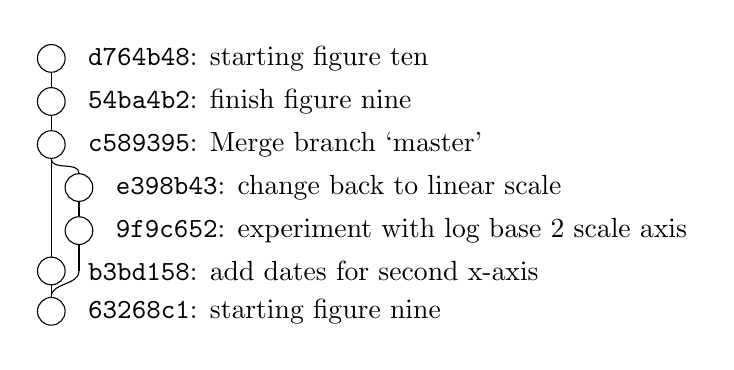
\begin{tikzpicture}
\tikzstyle{commit}=[draw,circle,fill=white,inner sep=0pt,minimum size=10pt]
\tikzstyle{clabel}=[right,outer sep=1em]
\tikzstyle{every path}=[draw]
\matrix [column sep={1em,between origins},row sep=\lineskip]
{
 
\commit{d764b48}{starting figure ten} & \\
\commit{54ba4b2}{finish figure nine} & \\
\commit{c589395}{Merge branch `master'} & \\
 & \commit{e398b43}{change back to linear scale} \\
 & \commit{9f9c652}{experiment with log base 2 scale axis} \\
\commit{b3bd158}{add dates for second x-axis} & \ghost{branch1} \\
\commit{63268c1}{starting figure nine} & \\
};
 
%% connections
 
\connect{63268c1}{b3bd158};
\connect{63268c1}{branch1};
\connect{branch1}{9f9c652};
\connect{9f9c652}{e398b43};
\connect{b3bd158}{c589395};
\connect{e398b43}{c589395};
\connect{c589395}{54ba4b2};
\connect{54ba4b2}{d764b48};
\end{tikzpicture}
\end{document}
